\section{Adaptation to Lance}
\label{lance-sec-adaptation}

As mentioned, the Lance approach grew out of challenges emerging from our
2005 field deployment at Reventador. Although this system was successfully
deployed, it exhibited several deficiencies which led to a significant loss
of data~\cite{volcano-osdi06}. 

The first problem is that the decision used to download a given signal was
based on a simplistic binary approach, based on the event-detection algorithm
running on each node. As a result, the system could not prioritize certain
events over others. The event-detector logic used a simple threshold scheme,
and as reported in~\cite{volcano-osdi06}, the threshold was set too low,
causing the network to trigger on less than 5\% of the actual seismic events.

The second problem was that following each trigger, the network initiated a
{\em nonpreemptive} download from every node in the network in a round-robin
fashion. This policy caused the system to devote resources to downloading
small precursor earthquakes that immediately preceded larger
eruptions~\cite{volcano-osdi06}. As a result, many such larger events were
not captured. 

Finally, our 2005 system made no attempt to manage energy. As a result,
the expected lifetime of the network is only about a week (using D-cell
batteries), necessitating frequent battery changes over a long deployment.
Clearly, this system could benefit from a prioritized approach to download
management that also considers energy costs to increase lifetime.

\subsection{Volcano Monitoring}
\label{lance-subsec-volcano}

To address these problems, we reimplemented our previous volcano monitoring
system using Lance. Many of the components of the original system, such as
multihop routing, time synchronization, reliable download protocol, and flash
storage interface, remained unchanged.  The node-level event detector was
replaced by an ADU summarization function, as described below. The base
station code for responding to correlated events was replaced with Lance's
optimizer and policy modules. Our deployment of the completed system at
Tungurahua volcano in August 2007 is discussed in
Section~\ref{lance-sec-deployment}.

\begin{figure}[t]
\begin{center}
\begin{tabular}{ll}
\raisebox{0.35in}{\parbox{0.05in}{\textbf{(a)}}} & 
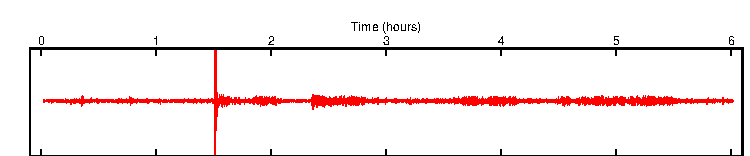
\includegraphics[width=0.95\hsize]{./figs/used/sixhour.pdf}
\vspace{-0.05in}\\
\raisebox{0.31in}{\parbox{0.05in}{\textbf{(b)}}} & 
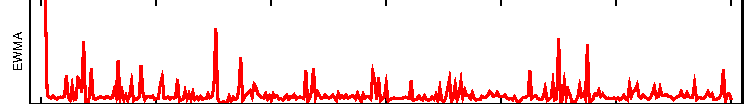
\includegraphics[width=0.95\hsize]{./figs/used/ewma.pdf}
\vspace{-0.05in}\\
\raisebox{0.32in}{\parbox{0.05in}{\textbf{(c)}}} & 
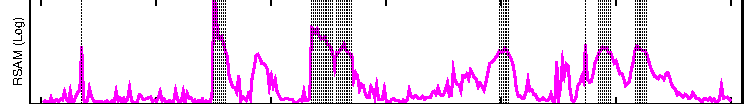
\includegraphics[width=0.95\hsize]{./figs/used/rsam.pdf}
\end{tabular}
\end{center}

\caption{\textbf{Comparing Two Node Utility Calculators:} Shown in relation
to the 6~hour data trace, subplot (a), are the output of the two candidate
node utility calculators described in Section~\ref{lance-subsec-volcano}
with dotted lines identifying the 50 highest-utility data units computed by
each detector. Subplot (b) shows the EWMA detector, which is good at
detecting event onsets; (c) shows the RSAM detector, which offers a better
indication of the overall strength of volcanic activity. Most of the 50 top
ADUs identified by the RSAM detector occur during long-period events, such as
volcanic tremor. Since the stated goal of the volcano monitoring application
was to extract short-period events we chose the EWMA detector for the
majority of our evaluation.}

\label{lance-fig-nucplot}
\end{figure}

The original system was intended to detect correlated seismic events from
across the network and download data from all nodes, regardless of whether
every node detected the event. This was based on a simple event detector that
computes two exponentially-weighted moving averages (EWMA) of the seismic
signal, with different gain settings; one EWMA represents the short-term
average and the other the long-term average. When the ratio between these two
averages exceeds a threshold, an event detection message is sent to the base
station. Subsequent triggers are suppressed for a short duration afterwards.

This policy is straightforward to implement in Lance by using the ``ratio of
two averages'' as the node-level summarization function.  Rather than
performing thresholding at the node level, we report the maximum ratio over
the ADU as its value, allowing Lance to prioritize different events. The base
station's policy modules are configured as shown in
Section~\ref{lance-sec-example-policies}, using a chain of {\tt filter}, {\tt
correlated}, and {\tt spacespread} to implement the equivalent of the event
triggering policy used in the original system. Note that the Lance version of
the system differs from the original in that download management is
value-driven rather than FIFO. Also, Lance can download ADUs from different
events out of order, avoiding the nonpreemptive download problems of the
earlier system.

While our original system was designed to capture short earthquakes, were
also interested in determining whether Lance could be used to capture
different types of volcanic activity. For this, we make use of the Real-Time
Seismic Amplitude Measurement (RSAM)~\cite{rsam}, which computes the average
seismic amplitude over a given time window.  Intuitively, RSAM measures the
total amount of ground shaking caused by earthquakes and tremor, and is often
used by volcano observatories to characterize the overall level of seismic
activity.

Different summarization functions and policy modules can be used to implement
a wide range of geophysical monitoring systems with Lance. For example, a
hazard monitoring system could be configured to periodically report RSAM
values for all sensor nodes and download only the strongest events for
further analysis. By limiting downloads to those ADUs with RSAM above some
threshold, energy can be saved. In contrast, a scientific study that wishes
to perform earthquake localization~\cite{aki-richards-80} or tomographic
inversion~\cite{lees-lindley-94} would prefer to download only small
earthquakes with clearly delineated onsets, which can be used to determine
the velocities of seismic waves. Likewise, a researcher studying explosive
events would prefer to download only seismic events with a corresponding
infrasonic component, since non-explosive earthquakes should not generate any
infrasound.

% MDW: I am commenting this out since it overlaps too much with the
% Pixie paper.
%\subsection{Motion analysis}
%
\subsection{Other Application Domains}

We believe that Lance can be used to benefit many applications that make use
of high-resolution signals delivered over a bandwidth-limited wireless
network. These applications require high data rates, precluding continuous
data collection, and rely on classification techniques to determine which
signals to download. Two examples are given below.

{\bf Structural monitoring:}
Structural monitoring systems collect vibration
waveforms from a building, bridge, or other structure in order to
study structural properties and seismic response.
In previous systems~\cite{netshm-emnets05,ggb-ipsn07}, data collection
has been triggered manually or on a simple periodic schedule. Instead,
Lance can be used to prioritize signals following an earthquake or 
forced excitation of the structure, similar to the EWMA and RSAM
functions described earlier. To save energy, the system could choose a
subset of nodes from which to download data to achieve a good spatial
distribution across the structure. The size of the subset could be
chosen depending on the strength of the excitation. In addition, 
policy modules can be used to perform periodic downloading of ADUs 
from each sensor for calibration, as well as to determine whether 
each sensor is still functioning properly.

{\bf Animal habitat monitoring:}
Habitat monitoring applications that deploy high-bandwidth sensors, such as
microphones or cameras, are good candidates for prioritized data extraction. 
An example application may attempt to download interesting audio signals
facilitating offline species classification or 
localization~\cite{girod-ipsn07}. The summarization function could
involve either a triggered event detector, an audio waveform
classifier, or motion detector from a series of camera images~\cite{cyclops}.

At the base station, policy modules can use offline knowledge of node
positions to modify the initial ADU value. One approach might enhance
spatial coverage by prioritizing data collection from nodes nearby the
source of the signal. Another could reject noise by deprioritizing signals
detected by only one node. For example, if fewer than three nodes
report an audio event, it is impossible to perform acoustic
localization and Lance need not waste bandwidth on the signal.
Policy modules can take other metrics into account as well, 
such as the SNR of the recorded signal or the time of day (e.g.,
reducing confidence in camera images taken at night).

Another application domain that we are exploring is motion
analysis of patients with movement disorders, such as Parkinson's
Disease~\cite{parkinsons-embs07}. In this context, up to ten sensor nodes
equipped with triaxial accelerometers and gyroscopes are placed on the
patient's limb segments (two each on the arms and legs plus one each
on the torso and waist), collecting high-resolution data at rates up to 100~Hz
or more. The goal is to capture data from the body
sensor network during periods of dyskinesia (abnormal movements) or
bradykinesia (slowness of movement) associated with the disease. 
The base station will typically 
be a laptop located in the home, and as such will experience a wide 
variation in bandwidth to the body sensor network (including
disconnections), depending on the patient's location.

Use of low-power wireless sensors keeps the size and weight
of each device down: for example, the wearable sensor node described
in~\cite{parkinsons-embs07} measures $44 \times 20 \times 13$~mm and
weighs just 10~g. 
While the sensor network is not spatially distributed, and
all nodes are within a single radio hop of each other, the data rates
greatly exceed the radio channel bandwidth: a single node will 
consume more than a quarter of the best-case radio capacity, assuming
no protocol overhead or retransmissions. 

We are currently developing a sensor network for motion analysis,
making use of Lance to drive the storage and bandwidth management.
Each sensor node computes a series of high-level {\em features} from
the raw sensor data, such as peak amplitude, maximum entropy, and
RMS. The node prioritization function assigns higher priority to 
features appearing to represent abnormal movement. The raw signal 
is also stored as separate ADUs with lower priority than the features,
allowing Lance to restrict downloads of the raw data to periods
with a strong radio link to the sensors. During periods of
disconnection, nodes will buffer ADUs for later transmission; the
wearable sensors we are using support a large (up to 2~GByte) flash
memory for this purpose. Priority modules at the base station can 
estimate the available bandwidth to the body sensors, based on radio
link quality, and prioritize downloads accordingly. Although this
system is still under development, Lance's core mechanisms and policy
modules appear to be a good fit for this application.

